\documentclass[11pt]{article}
\usepackage[utf8]{inputenc}
\usepackage[T1]{fontenc}
\usepackage{amsmath, amssymb, amsthm}
\usepackage{graphicx}
\usepackage{cite}
\usepackage{booktabs}
\usepackage{tikz}
\usepackage{hyperref}
\usetikzlibrary{shapes.geometric, arrows, positioning}

\title{Welcome to Your Modern LaTeX Workspace}
\author{Corca}
\date{\today}

\begin{document}

\maketitle

\begin{abstract}
This document demonstrates the power of running LaTeX directly in your browser. By combining high-speed execution with smart editing features, we provide a professional typesetting environment that requires zero installation and offers instant feedback.
\end{abstract}

\section{Introduction}
LaTeX has been the gold standard for scientific typesetting for decades. Recently, the advent of WebAssembly (WASM) has enabled the migration of these heavy-duty desktop applications to the web. Our platform utilizes the latest TeX Live 2025 distribution, providing over 4,000 packages and the most stable pdfTeX kernel to date. 

One of the key features of this sample is the seamless resolution of cross-references and bibliography. When a user edits the \texttt{.bib} file, the system automatically triggers a BibTeX run followed by necessary recompilations.


\section{Why it's so Fast: The Engine in Your Browser}
Traditionally, LaTeX requires a large installation on your computer or a slow connection to a remote server. This editor takes a different approach by running a full LaTeX engine \textit{locally} in your browser.

\begin{itemize}
    \item \textbf{No Server Latency:} Since the compilation happens on your own device, there's no need to wait for data to travel across the internet.
    \item \textbf{Instant Updates:} Small changes to your document appear in the PDF preview almost immediately.
    \item \textbf{Smart Resource Management:} Only the styles and fonts you actually use are downloaded, saving time and bandwidth.
\end{itemize}

\section{Smart Editing: Your Intelligent Assistant}
Writing LaTeX commands can be tricky. Our integrated \textbf{Language Server Protocol (LSP)} acts like an intelligent assistant that understands your document as you write it.

\begin{description}
    \item[Auto-completion:] Start typing a command like \texttt{\textbackslash graph...} and press Tab to complete it automatically.
    \item[Instant Information:] Hover your mouse over any command to see what it does and how to use it.
    \item[Real-time Feedback:] Errors are underlined in red with helpful messages, allowing you to fix mistakes as soon as they happen.
    \item[Smart Navigation:] Click on a citation like \cite{knuth1984tex} or a figure reference to jump directly to its source.
\end{description}

\section{Beautiful Mathematics}
LaTeX is the world standard for mathematical documents. It handles everything from simple fractions to complex physics equations with ease:
\begin{equation}
i\hbar \frac{\partial}{\partial t}\Psi(\mathbf{r},t) = \left [ -\frac{\hbar^2}{2m}\nabla^2 + V(\mathbf{r},t)\right ] \Psi(\mathbf{r},t)
\end{equation}

\section{Vector Graphics with TikZ}
You can create diagrams directly within your document using the TikZ package. Because they are defined mathematically, these graphics remain perfectly sharp at any zoom level.

\begin{figure}[h]
\centering
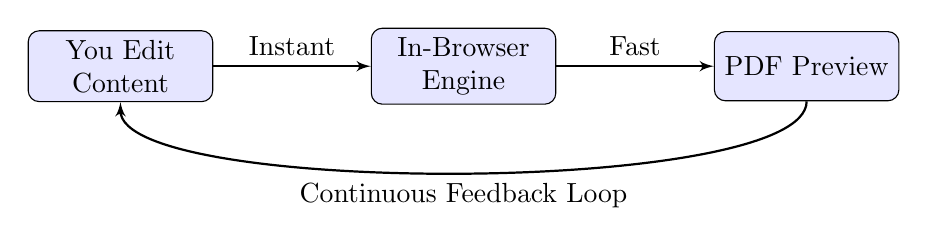
\begin{tikzpicture}[
    auto,
    block/.style={rectangle, draw, fill=blue!10, text width=6em, text centered, rounded corners, minimum height=2.5em},
    line/.style={draw, -latex', thick}
]
    \node [block] (edit) {You Edit Content};
    \node [block, right=2cm of edit] (wasm) {In-Browser Engine};
    \node [block, right=2cm of wasm] (pdf) {PDF Preview};
    
    \path [line] (edit) -- node {Instant} (wasm);
    \path [line] (wasm) -- node {Fast} (pdf);
    \draw [line] (pdf.south) .. controls +(down:1.2cm) and +(down:1.2cm) .. (edit.south) node [below, midway] {Continuous Feedback Loop};
\end{tikzpicture}
\caption{The real-time feedback loop enabled by local execution.}
\label{fig:loop}
\end{figure}

\section{Getting Started}
\autoref{fig:loop} shows the rendering pipeline and how changes to the document immediately update the output.
Simply start typing in the editor on the left. Any changes you make will be saved automatically, and the PDF on the right will update to reflect your work. Happy writing!

\bibliographystyle{plain}
\bibliography{refs}

\end{document}
